% vim: set tw=0:
\documentclass{beamer}
\usepackage{graphicx}
\usepackage{hyperref}
\hypersetup{pdfborder={0 0 0 0}}

% Reasonable themes:
% Antibes Bergen Berkeley Berlin Frankfurt Goettingen Ilmenau Luebeck Malmoe
% Montpellier PaloAlto Rochester Singapore Szeged Warsaw bars boxes
% compatibility default lined plain shadow sidebar split tree
% And these ones include the author's name on every slide:
% Berkeley

% Declare themes.
\mode<presentation>
\usetheme{UWHEP}

% Personal macros.
\newcommand{\email}[1]{{\texttt #1}}
\newcommand{\newframe}[1]{\section{#1}
    \frametitle{\sc{#1}}}
\newcommand{\subframe}[1]{\subsection{#1}
    \frametitle{\sc{#1}}}
\newcommand{\supers}[1]{\ensuremath{^\textrm{#1}}}
\newcommand{\subs}[1]{\ensuremath{_\textrm{#1}}}
\newcommand{\ca}{\ensuremath{\sim}}
\renewcommand{\email}[1]{\href{mailto:#1}{\nolinkurl{#1}}}

% Author information.
\title{T2 Status}
\author[Maier, Mohapatra]{
    Will Maier \and Ajit Mohapatra\\
    {\tt wcmaier@hep.wisc.edu}\\
    {\tt ajit@hep.wisc.edu}}
\institute[Wisconsin]{University of Wisconsin - High Energy Physics}
\date{2010.07.20}
\logo{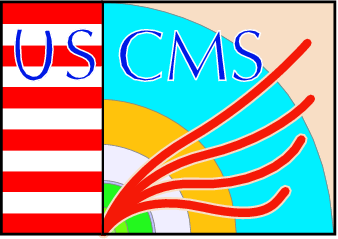
\includegraphics[height=0.6cm]{../../../Graphics/USCMS_logo.png}\hspace{.1cm}
\includegraphics[height=0.75cm]{../../../Graphics/UW_logo.png}}

\begin{document}

\begin{frame}
    \titlepage
\end{frame}

%\section{Overview}
%\begin{frame}
%    \tableofcontents
%\end{frame}

\section{Facilities}
\subsection{Software and Storage}
\begin{frame}
\frametitle{}

\begin{itemize}
	\item 32 2x8 core Opteron 6136 servers finally shipping (still)
	\begin{itemize}
		\item Vendor found that 8/32 servers randomly rebooted during stressapptest~\footnote{\url{http://code.google.com/p/stressapptest/}}
		\item Replacing all power supplies, retesting\ldots{}expect to ship this week
	\end{itemize}
	\item Tweaked kernel knobs to reduce SRM timeouts in PhEDEx
	\begin{itemize}
		\item Alex Sim (OSG Storage) suggested increasing {\tt net.core.somaxconn} and {\tt net.core.netdev\_max\_backlog} (had been at default)
		\item No non-PNFS related timeouts since
	\end{itemize}
	\item Preparing next round of compute/storage purchases
	\item Debugged CRAB routing to our site
	\item User merge jobs mysteriously locking up login machines
	\item Fixed stalled CEMon (which also fixed missing SAM tests)
	\item 2010.07.18: gatekeeper locked up
	\begin{itemize}
		\item Looked like "zombie" problem, so applied sysctl fix there as well
	\end{itemize}
	\item Integrating site-level monitoring
\end{itemize}
\end{frame}

\subsection{Production and Monitoring}
\begin{frame}
\frametitle{}

\begin{itemize}
	\item JobRobot: OK
	\item SAM: OK
	\item RSV: OK
	\item PhEDEx:
	\begin{itemize}
		\item LoadTest instance is running OK with release 3\_1\_1 on the new SL5 server 
		\item Moving Prod instance to SL5 now that ICHEP rush is over; Loadtest instance will move next
		\item No major issues with data xfers to Wisconsin
	\end{itemize}
	\item MC Production:
	\begin{itemize}
		\item Production for ICHEP rush is over, now getting back to normal mode
		\item Not very many requests since last week except LHE/Alpgen samples (\ca{}~200M)
		\item Moving to new ProdAgent release, usual WF testing
	\end{itemize}
\end{itemize}
\end{frame}

\end{document}
